\documentclass{article}
\usepackage{graphicx}
\usepackage[english,greek]{babel}
\usepackage[utf8x]{inputenc}
\usepackage{amsmath}
\usepackage{relsize}
\usepackage{enumerate}
\usepackage[parfill]{parskip}
\usepackage{graphicx}

\makeatletter
\renewcommand*\env@matrix[1][*\c@MaxMatrixCols c]{%
  \hskip -\arraycolsep
  \let\@ifnextchar\new@ifnextchar
  \array{#1}}
\makeatother

\begin{document}

\title{\vspace{-3.5cm}\textbf{Προστασία και Ασφάλεια Υπολογιστικών Συστημάτων \\ΕΑΡΙΝΟ 2018\\ \textlatin{Project \#}1}}
\author{Λάμπρου Ιωάννης \\1115201400088\\\\ Στεφανίδης - Βοζίκης Κωνσταντίνος \\1115201400192}

\maketitle
\section*{\textlatin{Defense}}
\subsection*{\textlatin{SQL Injection}}
Το \textlatin{openeclass}, στην μορφή που το παραλάβαμε, πριν τροποποιήσουμε τον κώδικά του, 
βασιζόταν κυρίως στην λειτουργία των \textlatin{magic quotes} για άμυνα έναντι \textlatin{SQL Injections},
αλλά επιπλέον είχαν δημιουργηθεί οι συναρτήσεις \textlatin{escapeSimple()} και \textlatin{autoquote()} οι
οποίες έκαναν έλεγχο αν τα \textlatin{magix quotes} ήταν ενεργοποιημένα στον \textlatin{server}, και, αν
όχι, τότε εφάρμοζαν τις \textlatin{mysql\_real\_escape\_string()} ή \textlatin{mysql\_escape\_string()} και
\textlatin{addslashes()} στα ορίσματά τους αντίστοιχα. Δυστυχώς οι συναρτήσεις αυτές όμως δεν
χρησιμοποιούνταν σε πάρα πολλά μέρη όπου μια εξωτερική μεταβλητή
έμπαινε σε \textlatin{SQL query}. Ακόμα, οι σελίδες του \textlatin{admin} ήταν απροστάτευτες, δικαιολογημένα.\\
Εμείς, για προστασία, αφού τα \textlatin{prepared statements (libraries MySQLi, PDO)} δεν επιτρέπονται στα
πλαίσια της εργασίας, επιλέξαμε την επόμενη καλύτερη λύση, την χρήση της συνάρτησης
\textlatin{mysql\_real\_escape\_string()}.
Η συνάρτηση αυτή εφαρμόστηκε σε κάθε μεταβλητή η οποία γινόταν \textlatin{append}
σε \textlatin{sql query string}, σε μερικές περιπτώσεις αντικαθιστώντας τη χρήση των υπολοίπων παραπάνω
συναρτήσεων. Ακόμη να σημειωθεί πως η λειτουργικότητα της εφαρμογής δεν άλλαξε, αφού επιτρέπεται ακριβώς το


\subsection*{\textlatin{XSS}}
Αρχικά, το \textlatin{openeclass} είχε πολύ λίγη προστασία ενάντια σε \textlatin{XSS}
(ειδικά στα \textlatin{modules} που κληθήκαμε να προστατεύσουμε), με εξαίρεση τις σελίδες του
\textlatin{admin} οι οποίες ήταν πολύ καλά προστατευμένες, (είχε οριστεί ακόμα και η συνάρτηση
\textlatin{q()} ως συντόμευση της \textlatin{htmlspecialchars()}) Για την προστασία της εφαρμογής, τώρα πια
κάθε ματαβλητή η τιμή της οποίας εμφανιζόταν στον τελικό \textlatin{html} κώδικα, (γινόταν
\textlatin{append} στο \textlatin{\$tool\_content}) φιλτράρεται πρώτα μέσω της κλίσης της συνάρτησης
\textlatin{htmlspecialchars()} είτε προέρχεται από ερώτηση στη βάση ή κάποιο αρχείο, είτε από τον χρήστη της
εφαρμογής μέσω \textlatin{GET} ή \textlatin{POST}. Πρέπει να τονιστεί το γεγονός ότι ποτέ τα
\textlatin{inputs} δεν φιλτράρονται κατά την αποθήκευση, αλλά μόνο όταν πρόκειται να εμφανιστούν σε
\textlatin{html} κώδικα.


\subsection*{\textlatin{CSRF}}
Όσον αφορά την άμυνα για τις επιθέσεις \textlatin{CSRF}. Ποστατευθήκαμε βάζοντας \textlatin{CSRF tokens}
σε κάθε φόρμα ή οποία προκαλεί αλλαγές στην σελίδα. Σε κώδικα \textlatin{PHP} ή άμυνα μοιάζει κάπως
έτσι:\\
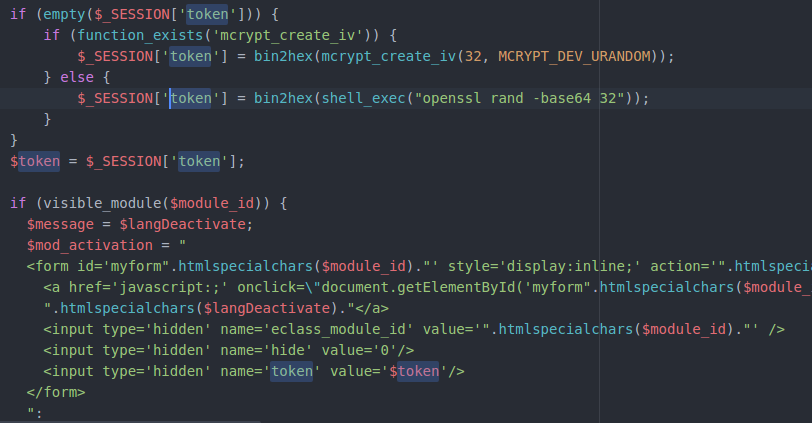
\includegraphics[scale=0.5]{csrf}\\
Πρώτα ενεργοποιούμε ενα \textlatin{token} και κατόπιν το βάζουμε ως \textlatin{hidden field} στην
φόρμα που μας ενδιαφέρει. Ο έλεγχος εγκυρότητας γίνεται ως εξης:\\
\textlatin{if (isset(\$\_POST['hide']) and \$\_POST['hide'] == 0 and !empty(\$\_POST['token']) and
(strcmp(\$\_SESSION['token'], \$\_POST['token']) === 0))}\\
Η ίδια λογική άμυνας υπάρχει σε κάθε φόρμα της ιστοσελίδας (η οποία προκαλεί αλλαγές).
Επίσης, επειδή δεν υπάρχει άμυνα έναντι επιθέσεων \textlatin{CSRF} σε \textlatin{GET requests}, διάφορα
\textlatin{GET} που άλλαζαν την σελίδα αλλάχθηκαν σε \textlatin{POST} ώστε να γίνει η ίδια άμυνα.
Ένα παράδειγμα είναι η διαγραφή χρήστη από την σελίδα του \textlatin{admin}.

\subsection*{\textlatin{RFI}}









\section*{\textlatin{Attack}}








\subsection*{\textlatin{SQL Injection}}
Για επίθεση \textlatin{SQL Injection}, σε περίπτωση που βρισκόταν κάποιο \textlatin{vulnerability}, θα υπήρχε η δυνατότητα να βρεθεί το \textlatin{hashed password} του \textlatin{drunkadmin}, ή να μάθουμε το όνομα του \textlatin{directory} που δημιουργείται για την αποθήκευση των εργασιών ή τα ονόματα των αρχείων που έχουμε στείλει για ανταλλαγή αρχείων, έτσι ώστε να προσπαθήσουμε να τα κάνουμε \textlatin{request} και να επιτύχουμε \textlatin{RFI}. Ακόμη μια καλή στρατιγική θα ήταν να μετατρέψουμε τον χρήστη μας σε \textlatin{admin}, αλλάζοντας το \textlatin{userid} του \textlatin{admin} σε κάτι εκτός από 1 και κάνοντας το δικό μας 1, αφού η εφαρμογή θεωρεί ότι ο χρήστης με \textlatin{userid} 1 είναι ο \textlatin{admin}. Σημειώνεται πως δεν γνωρίζουμε το δικό μας \textlatin{userid} αλλά θα μπορούσαμε είτε να το μάθουμε, αν έχουμε βρει \textlatin{SQL Injection vulnerability}, είτε να μαντέψουμε, αφού δεν είναι και πολλές περιπτώσεις, ανάλογα και με τους συνολικούς χρήστες της εφαρμοφής. Δυστυχώς η αντίπαλη ομάδα ήταν καλά προστατευμένη έναντι σε \textlatin{SQL Injection} και δεν βρέθηκαν \textlatin{vulnerabilities}. Με την προσθήκη, για παράδειγμα, σε ένα \textlatin{search keyword} του \textlatin{string ' AND '1' = '1}   





\subsection*{\textlatin{XSS}}
Αντίθετα, η αντίπαλη εφαρμογή είχε πολλές ευπάθειες σε \textlatin{XSS attacks}. Aρχικά, στην ανταλλαγή αρχείων, το όνομα αλλά και η περιγραφή 

\subsection*{\textlatin{CSRF}}
Η σελίδα ήταν γενικά πολύ ευάλωτη σε επιθέσεις \textlatin{CSRF}. Η πρώτη
επίθεση που δοκιμάστηκε και ήταν επιτυχής ήταν η \textlatin{malicious} εισαγωγή
μαθήματος απο τον διαχειριστή ο οποίος ανυποψίαστος πάτησε ένα λίνκ που του στειλαμε με
\textlatin{email}. Άλλες επιθέσεις με \textlatin{CSRF} δεν πραγματοποιήθηκαν καθώς μετά
κάναμε ολοκληρωτικό \textlatin{deface} της σελίδας οπότε και το \textlatin{CSRF} ήταν πιο
ανίσχυρο από τις άλλες επιθέσεις. Παρόλα αυτά είχαν βρεθεί ευπάθειες και είχαν σχεδιαστεί
επιθέσεις σε μια σωρεία λειτουργιών όπως η διαγραφή εργασίας, διαγραφή μαθήματος, διαγραφή
χρήστη, δημιουργία ανακοίνωσης, δημιουργία εργασίας σε μάθημα.



\subsection*{\textlatin{RFI}}
\end{document}
